\documentclass[a4paper,12pt]{report}

\usepackage{alltt, fancyvrb, url}
\usepackage{graphicx}
\usepackage[utf8]{inputenc}
\usepackage{float}
\usepackage{hyperref}

\usepackage{amssymb}
\usepackage{amsmath}

% Questo commentalo se vuoi scrivere in inglese.
\usepackage[italian]{babel}

\usepackage[italian]{cleveref}

%\linespread{1.25} % Imposta l'interlinea di x volte la dimensione del carattere

\title{Teoria dei numeri \\ applicata alla Crittografia}

\author{Giosuè Giocondo Mainardi\\ (n.0000933566)}
\date{\today}

\begin{document}

\maketitle

\tableofcontents
\chapter{Introduzione}
La \textbf{crittografia} è fondamentale per garantire la sicurezza delle comunicazioni digitali, proteggendo la \emph{confidenzialità, l'integrità e l'autenticità} dei dati scambiati. 
Molti degli algoritmi crittografici più diffusi e robusti si basano su solidi principi matematici derivanti dalla \textbf{teoria dei numeri}. 

Sebbene in passato crittografia e matematica fossero viste come discipline separate, con \emph{G.H. Hardy} che nel 1940 vedeva la matematica come una scienza neutra, pura e gentile,
che non si schiera e non ha applicazioni dirette, l'avvento dell'informatica ha dimostrato il loro stretto legame. 

La teoria dei numeri, con lo studio delle proprietà dei numeri interi, dei \textbf{numeri primi} e delle loro interazioni, è diventata un pilastro portante per lo sviluppo di sistemi crittografici sicuri.

La \textbf{fattorizzazione in numeri primi}, il \textbf{logaritmo discreto} e le \textbf{equazioni diofantee} sono solo alcuni dei concetti chiave della teoria dei numeri che trovano 
applicazione nella crittografia moderna. Algoritmi rivoluzionari come \emph{RSA} e \emph{Diffie-Hellman}, basilari per la crittografia a chiave pubblica, sfruttano questi principi 
per garantire elevati livelli di sicurezza. La casualità è una caratteristica fondamentale in crittografia, eppure, come sottolineava \emph{Von Neumann}, 
``Chiunque consideri metodi aritmetici per produrre cifre casuali è, ovviamente, in stato di peccato'', evidenziando l'impossibilità di ottenere vera casualità in aritmetica. 
Tuttavia, la teoria dei numeri offre proprietà ideali per nascondere e proteggere informazioni, come la difficoltà nel risolvere alcuni problemi aritmetici nonostante la loro apparente semplicità.

In questa relazione, esploreremo nel dettaglio il legame inscindibile tra crittografia e teoria dei numeri, analizzando le principali applicazioni di quest'ultima nella protezione dei dati digitali. 
Verranno approfonditi concetti come la fattorizzazione, il logaritmo discreto e le equazioni diofantee, al fine di comprendere appieno il \textbf{ruolo cruciale} svolto dalla matematica nella \textbf{sicurezza informatica}.
%
%
%
%
\chapter{Fondamenti della teoria dei numeri}
È importante fornire prima basi teoriche matematiche per comprendere il funzionamento degli algoritmi che andremo a trattare.

La teoria dei numeri è lo studio dei numeri interi, e delle loro proprietà. L'insieme dei numeri interi è $\mathbb{Z}$ e contiene tutti i numeri interi positivi e negativi, insieme allo zero.
\begin{quote}
	\centering
	..., -5, -4, -3, -2, -1,  0,  1,  2,  3,  4,  5, ...
\end{quote}

\section{Definizioni}

\subsection*{Numero primo}
Un numero primo è un numero intero \( p > 1 \) che ha esattamente due divisori: 1 e \(p\) (se stesso).

\textbf{Esempi}: ogni numero a sinistra nella seguente tabella è primo.
\[\begin{array}{ll}
3 & = 2 + 1 \\
7 & = 2 \cdot 3 + 1 \\
31 & = 2 \cdot 3 \cdot 5 + 1 \\
211 & = 2 \cdot 3 \cdot 5 \cdot 7 + 1 \\
2311 & = 2 \cdot 3 \cdot 5 \cdot 7 \cdot 11 + 1 \\
\end{array}\]
Questo schema non continua indefinitamente, ma qualcosa di simile funziona.

Occorre però ricordare che Euclide ha dimostrato che esistono infiniti numeri primi. \cite{stein2008}

Inoltre, si fa notare che il più grande numero primo conosciuto\footnote{Largest Know Prime Number:7 dicembre 2018 da Patrick Laroche} è \[2^{82,589,933} - 1\]
e ha quasi 25 milioni di cifre.

\subsection*{Numero composto}
Un numero composto è un numero intero \( n > 1 \) che ha almeno un altro divisore, oltre 1 e \( n \) (se stesso).

\section{Concetti Fondamentali}
\subsection*{Fattorizzazione}
La fattorizzazione è il processo di scomposizione di un numero intero \( n \) in un prodotto di numeri primi. 

\textbf{Formalmente}: dato un numero intero \( n \), la fattorizzazione di \( n \) è data dalla rappresentazione: 

\[ n = p_1^{e_1} \cdot p_2^{e_2} \cdot \ldots \cdot p_k^{e_k} \]

dove \( p_1, p_2, \ldots, p_k \) sono numeri primi distinti e \( e_1, e_2, \ldots, e_k \) sono esponenti positivi.

\subsection*{Divisibilità e criteri di divisibilità}

Un numero \(a\) è divisibile per un numero \(b\) se il resto della divisione di \(a\) per \(b\) è zero. In altre parole, se esiste un numero intero \(k\) tale che \(a = b \cdot k\), allora \(a\) è divisibile per \(b\).

Alcuni criteri di divisibilità comuni sono:
\begin{itemize}
	\item \textbf{Criterio della divisibilità per 2}: Un numero è divisibile per 2 se la sua ultima cifra è pari, cioè se termina con 0, 2, 4, 6 o 8.
	
	\item \textbf{Criterio della divisibilità per 3}: Un numero è divisibile per 3 se la somma delle sue cifre è divisibile per 3.
	
	\item \textbf{Criterio della divisibilità per 5}: Un numero è divisibile per 5 se termina con 0 o 5.
	
	\item \textbf{Criterio della divisibilità per 7}: Un numero è divisibile per 7 se il numero ottenuto sottraendo dal doppio della cifra delle unità il numero ottenuto togliendo la cifra delle unità è divisibile per 7.

	\item \textbf{Criterio della divisibilità per 11}: Un numero è divisibile per 11 se la differenza tra la somma delle cifre in posizione pari e la somma delle cifre in posizione dispari è un multiplo di 11(compreso lo 0).

\end{itemize}

\subsection*{Massimo comune divisore (MCD)}
Il massimo comune divisore di due numeri interi \( a \) e \( b \), denotato come 
\[ \mathbb{MCD}(a, b) \] 
ed è il più grande numero intero che divide entrambi \( a \) e \( b \) senza lasciare resto.

\subsection*{Minimo comune multiplo (mcm)}
Il minimo comune multiplo di due numeri interi \( a \) e \( b \), denotato come 
\[ \mathrm{mcm}(a, b) \]
ed è il più piccolo multiplo comune di \( a \) e \( b \).

\subsection*{Numeri coprimi}
Due numeri interi sono definiti come \textbf{coprimi} (o primi tra loro) se il loro massimo comune divisore (MCD) è uguale a 1. 

\textbf{Formalmente}: dati due numeri interi \(a\) e \(b\), essi sono coprimi se e solo se:
\[\mathbb{MCD}(a, b) = 1\]

\chapter{Aritmetica Modulare}

L'aritmetica modulare è un ramo fondamentale della teoria dei numeri che studia le operazioni aritmetiche sui resti delle divisioni intere. Questo capitolo esplora i concetti chiave dell'aritmetica modulare necessari per comprendere molti algoritmi crittografici moderni.

\section{Definizioni} 
\subsection*{Operatore modulo} Dato un numero intero $a$ e un modulo $n$, numero intero positivo, il "resto della divisione di $a$ per $n$" è il valore che rimane quando $a$ è diviso per $n$. Questo valore è sempre compreso tra 0 e $n-1$, inclusi.

Simbolicamente, possiamo esprimere il resto della divisione di $a$ per $n$ come:

\[ a \mod n \]

dove "mod" è l'operatore modulo.

\subsection*{Insieme modulo \( \mathbb{Z}_n\)}
Si sceglie un numero intero positivo \(n\), chiamato modulo, che determina l'insieme dei resti modulo \(n\). 
Questo insieme è denotato come \(\mathbb{Z}_n\)  , ed è composto da tutti i numeri interi che vanno da 0 a \(n-1\).

\textbf{Formalmente}: \[\mathbb{Z}_n = \{0, 1, 2, \ldots, n-1\}\]

\subsection*{Gruppo moltiplicativo \(\mathbb{Z}_n^*\)}
Un insieme modulo che contiene solo numeri coprimi rispetto al modulo dato è noto come gruppo moltiplicativo modulo \(n\), indicato con \(\mathbb{Z}_n^*\) o \((\mathbb{Z}/n\mathbb{Z})^*\). 
Questo gruppo è composto da tutti gli interi positivi minori di \(n\) che sono coprimi con \(n\).

\textbf{Formalmente}: \[\mathbb{Z}_n^* = \{a \in \mathbb{Z}_n : \text{MCD}(a, n) = 1\}\]

\subsection*{Funzione Totiente di Eulero} \label{sec:totiente}
La funzione totiente di Eulero, indicata con $\phi(n)$, conta il numero di interi positivi minori o uguali a $n$ che sono coprimi con $n$, ovvero che non hanno fattori comuni con $n$ eccetto $1$. 

\textbf{Formalmente}:\[\phi(n) = |\{a \in \mathbb{Z}_n : \mathbb{MCD}(a, n) = 1\}| = |\mathbb{Z}_n^*|\]
\section{Congruenza Modulare}

Data una coppia di interi $a$ e $b$, e un intero positivo $n$ detto \textbf{modulo}, diciamo che $a$ è congruo a $b$ modulo $n$, denotato come:

$$a \equiv b \pmod{n}$$

Se esistono interi $k_1$ e $k_2$ tali che:

$$a = k_1n + b$$
$$b = k_2n + a$$

In altre parole, $a$ e $b$ hanno lo stesso resto quando divisi per $n$. 

\subsection*{Classe di Resto}
L'insieme di tutti gli interi congrui a $a$ modulo $n$ è chiamato \textbf{classe di resto} o \textbf{classe di congruenza} di $a$ modulo $n$, denotata come \[[a]_n\]

\subsection*{Proprietà}
La relazione di congruenza gode delle seguenti proprietà:

\begin{enumerate}
    \item \textbf{Riflessività}: $a \equiv a \pmod{n}$ per ogni $a \in \mathbb{Z}$ e $n > 0$.
    \item \textbf{Simmetria}: Se $a \equiv b \pmod{n}$, allora $b \equiv a \pmod{n}$.
    \item \textbf{Transitività}: Se $a \equiv b \pmod{n}$ e $b \equiv c \pmod{n}$, allora $a \equiv c \pmod{n}$.
\end{enumerate}

\section{Operazioni Aritmetiche Modulari}
Le operazioni aritmetiche fondamentali (addizione, sottrazione, moltiplicazione ed esponenziazione) possono essere definite sull'insieme dei residui modulo $n$, denotato come $\mathbb{Z}_n$. Per $a, b \in \mathbb{Z}_n$:

\begin{enumerate}
    \item \textbf{Addizione modulare}:
    $$(a + b) \bmod n = r \quad \text{dove } r \in \mathbb{Z}_n \text{ è il resto della divisione di } a+b \text{ per } n$$
    
    \item \textbf{Sottrazione modulare}:
    $$(a - b) \bmod n = r \quad \text{dove } r \in \mathbb{Z}_n \text{ è il resto della divisione di } a-b \text{ per } n$$
    
    \item \textbf{Moltiplicazione modulare}:
    $$(a \cdot b) \bmod n = r \quad \text{dove } r \in \mathbb{Z}_n \text{ è il resto della divisione di } a \cdot b \text{ per } n$$
    
    \item \textbf{Esponenziazione modulare}:
    $$a^b \bmod n = r \quad \text{dove } r \in \mathbb{Z}_n \text{ è il resto della divisione di } a^b \text{ per } n$$
\end{enumerate}

Queste operazioni godono delle stesse proprietà dell'aritmetica ordinaria: commutativà per addizione e moltiplicazione, associatività, elementi neutri (0 per addizione, 1 per moltiplicazione) e inversi (modulo $n$).

\section{Inverso Moltiplicativo Modulare}

Un concetto cruciale è quello di \textbf{elemento invertibile modulo $n$}: 

un numero $a \in \mathbb{Z}_n$ è invertibile se esiste $b \in \mathbb{Z}_n$ tale che $ab \equiv 1 \pmod{n}$. $b$ è detto l'\textbf{inverso moltiplicativo} di $a$ modulo $n$, denotato come $a^{-1}$.

\subsection*{Esistenza dell'Inverso Moltiplicativo}
L'inverso moltiplicativo di $a$ modulo $n$ esiste se e solo se $a$ e $n$ sono coprimi, ovvero il loro massimo comune divisore $\mathbb{MCD}(a,n) = 1$. 

\subsection*{Calcolo dell'Inverso Moltiplicativo} \label{sec:inverso}
L'inverso moltiplicativo di $a$ modulo $n$ si può calcolare efficacemente tramite l'algoritmo euclideo esteso e che sfrutta l'equazione di Bezout:
\[ ax+ny=1 \]
In cui $x$ è l'inverso moltiplicativo di $a$ modulo $n$.

\section{Aritmetica Modulare sui Numeri Primi}

Le proprietà dell'aritmetica modulare si semplificano notevolmente quando il modulo $n$ è un numero primo $p$. In questo caso, l'insieme $\mathbb{Z}_p$ è un \textbf{campo}, ovvero ogni elemento non nullo è invertibile (\( |\mathbb{Z}_p| =|\mathbb{Z}_p^*| \)).

\subsubsection*{Piccolo Teorema di Fermat}

$$a^p \equiv a \pmod{p} \quad \forall a \in \mathbb{Z}$$

Questo significa che elevare un numero $a$ alla potenza $p$ modulo $p$ dà come risultato $a$ stesso.

È spesso espresso nella forma equivalente, con \(a\) che è un intero coprimo con \(p\):

\[a^{p-1} \equiv 1 \pmod{p}\quad,\quad con\quad \mathbb{MCD}(a,p)=1\]

Va notato che la prima espressione è in un certo senso più generale: è infatti valida per numeri interi arbitrari, come \(0\) o multipli di \(p\), che invece non rientrano nelle ipotesi della seconda.

\subsubsection*{Teorema di Eulero (Fermat generalizzato)}

$$a^{\phi(n)} \equiv 1 \pmod{n} \quad \text{se } \mathbb{MCD}(a,n) = 1$$

Dove $\phi(n)$ è la \textbf{funzione totiente di Eulero}, che conta il numero di interi positivi minori di $n$ e coprimi con $n$.
%
%
%
%
%
%
%
%
%
%
%
%
%
%
%
%
%
%
%
%
%
%
%
%
%
%
%
%
%
%
%
%
%
%
%
%
%
%
%
%
%
\chapter{Il Cifrario RSA}

\section{Introduzione}
Il cifrario RSA, introdotto dai crittografi Ron Rivest, Adi Shamir e Leonard Adleman nel 1977, rappresenta uno dei più importanti e diffusi algoritmi crittografici a chiave pubblica. 
Esso sfrutta le proprietà della teoria dei numeri e dell'aritmetica modulare per garantire la sicurezza delle comunicazioni. 
A differenza dei sistemi crittografici a chiave simmetrica, in cui la stessa chiave viene utilizzata per cifrare e decifrare i messaggi, il cifrario RSA utilizza due chiavi diverse, una pubblica e una privata.

\section{Principi Fondamentali}
Il cifrario RSA si basa su due principi fondamentali:

\begin{enumerate}
    \item La \textbf{difficoltà computazionale} di fattorizzare grandi numeri interi composti. Questo problema, noto come "problema della fattorizzazione intera", è uno dei problemi più difficili in teoria dei numeri e in crittografia. Anche se non è stato dimostrato essere NP-hard\footnote[1]{NP-hard significa che un problema è almeno tanto difficile quanto il problema più difficile in NP (nondeterministic polynomial time).}, non si conosce alcun algoritmo efficiente in grado di risolverlo in tempi ragionevoli per numeri sufficientemente grandi.
    \item La \textbf{facilità relativa di calcolare esponenziali modulari}, operazione che sta alla base del processo di cifratura e decifratura. Infatti, questa può essere eseguita in modo efficiente tramite tecniche come l'esponenziazione veloce.
\end{enumerate}

\section{Generazione delle Chiavi}
La generazione delle chiavi nel cifrario RSA segue i seguenti passi:

\begin{enumerate}
    \item Scegliere due numeri primi distinti $p$ e $q$ di grandi dimensioni.
    \item Calcolare $n = p \cdot q$, dove $n$ è chiamato modulo. La dimensione di $n$ determina la sicurezza del sistema crittografico.
    \item Calcolare $\phi(n) = (p - 1)(q - 1)$, dove $\phi$ è la funzione totiente di Eulero, vedi \ref{sec:totiente}.
    \item Scegliere un numero intero $e$ tale che $1 < e < \phi(n)$ e $\operatorname{MCD}(e, \phi(n)) = 1$. Il numero $e$ è chiamato esponente di cifratura. Tipicamente, si sceglie un valore piccolo per $e$, come $65537$ \footnote{Numero primo ha pochi bit impostati a 1, cosa che velocizza l'elaborazione}, per rendere più efficienti le operazioni di cifratura.
    \item Determinare $d$ tale che $d \cdot e \equiv 1 \pmod{\phi(n)}$. Il numero $d$ è chiamato esponente di decifratura. Esso può essere calcolato usando l'algoritmo di Euclide esteso, come specificato in \ref{sec:inverso}.
\end{enumerate}

La coppia $(e, n)$ rappresenta la chiave pubblica, mentre $(d)$ è la chiave privata. La chiave pubblica può essere ampiamente diffusa, mentre la chiave privata deve essere mantenuta segreta.

\subsection*{Determinazione dei numeri primi}
La scelta dei due numeri primi $p$ e $q$ è cruciale per garantire la sicurezza del cifrario RSA. 
Essi devono essere scelti in modo casuale e devono essere di dimensioni sufficientemente grandi per resistere a potenziali attacchi di forza bruta o di fattorizzazione.
I passi per la generazione di un numero primo "forte":

\begin{itemize}
    \item{Scelta della \textbf{dimensione} (n°bit).}
    \item{\textbf{Generazione Casuale} del numero.} 
    \item{\textbf{Verifica della Primalità}: ci sono diversi Test per verificare che il numero generato sia effettivamente primo, come il Test di Miller-Rabin o il Test di Fermat. \cite{stein2008}}
    \item{\textbf{Ripetizione}: Se il numero generato non è primo, si ripete il processo di generazione fino a ottenere un numero primo valido.}
    \item{\textbf{Utilizzo di Numeri Primi Sicuri}: In alternativa, si possono utilizzare numeri primi sicuri predefiniti, noti come numeri primi di Sophie Germain o numeri primi di Safeprimes. \cite{boneh2005}}
\end{itemize}

\subsection*{Specifiche Attuali della Lunghezza delle Chiavi RSA}

Ecco le specifiche attuali per la lunghezza delle chiavi RSA:

\begin{itemize}
    \item \textbf{1024 bit}: Considerata insicura per la maggior parte degli scopi. Non è più raccomandata per l'uso.
    \item \textbf{2048 bit}: Attualmente considerata sicura per la maggior parte degli scopi. Raccomandata per molti utilizzi.
    \item \textbf{3072 bit}: Fornisce un margine di sicurezza maggiore, utilizzata per esigenze di sicurezza più elevate.
    \item \textbf{4096 bit}: Utilizzata per esigenze di sicurezza molto elevate, anche se comporta operazioni più lente.
\end{itemize}

Queste raccomandazioni sono in linea con le linee guida fornite da organizzazioni come il NIST (National Institute of Standards and Technology)\cite{nist}.

\section{Cifratura e Decifratura}
Sia $m$ il messaggio in chiaro, rappresentato come un numero intero nel range $[0, n - 1]$. Per trasformare il messaggio in un numero intero, si possono utilizzare varie tecniche di codifica, come la rappresentazione ASCII o Unicode dei caratteri.

\begin{enumerate}
    \item La cifratura avviene calcolando $c \equiv m^e \pmod{n}$, dove $c$ è il testo cifrato.
    \item La decifratura avviene calcolando $m \equiv c^d \pmod{n}$.
\end{enumerate}

La sicurezza del cifrario RSA risiede nella difficoltà computazionale di fattorizzare $n$ in $p$ e $q$, dato che la conoscenza di $p$ e $q$ permette di calcolare $\phi(n)$ e quindi la chiave privata $d$. Pertanto, la scelta di numeri primi $p$ e $q$ sufficientemente grandi è cruciale per garantire la sicurezza del sistema.

\section{Applicazioni e Considerazioni sulla Sicurezza}
Il cifrario RSA trova applicazione in numerosi contesti, come la crittografia dei dati, la firma digitale, lo scambio di chiavi e l'autenticazione. Esso è ampiamente utilizzato in diversi protocolli di sicurezza, come SSL/TLS, PGP e molti altri.

Tuttavia, è importante sottolineare che la sicurezza del cifrario RSA basandosi sulla difficoltà di fattorizzare grandi numeri interi composti, con l'avanzamento della potenza di calcolo dei computer e lo sviluppo di nuovi algoritmi di fattorizzazione, potrebbe diventare necessario aumentare le dimensioni delle chiavi per mantenere un adeguato livello di sicurezza.

Inoltre, esistono altre potenziali vulnerabilità legate all'implementazione del cifrario RSA, come la scelta di numeri primi deboli, la gestione non sicura delle chiavi private e la possibilità di attacchi side-channel. Pertanto, è fondamentale seguire le best practice di sicurezza e utilizzare implementazioni affidabili e constantemente aggiornate del cifrario RSA.

\section{RSA a Chiave Multipla}

Il cifrario RSA a chiave multipla è un'estensione dell'algoritmo RSA standard progettata per consentire la cifratura di messaggi destinati a più destinatari utilizzando una singola chiave privata. In questa sezione, esploreremo le principali differenze e aggiunte rispetto a RSA standard.

\subsection{Generazione delle Chiavi}

Nel RSA a chiave multipla, vengono generate più coppie di chiavi pubbliche/ private, una per ogni destinatario. Sia \( (N_i, e_i, d_i) \) la \( i \)-esima coppia di chiavi generate, dove \( N_i \) è il modulo, \( e_i \) è l'esponente pubblico e \( d_i \) è l'esponente privato. Questo richiede una procedura di generazione delle chiavi più complessa rispetto alla generazione di una singola coppia di chiavi.

\subsection{Cifratura dei Messaggi}

Il mittente utilizza la propria chiave privata \( d_S \) per cifrare il messaggio \( M \). Il messaggio cifrato \( C \) viene quindi cifrato separatamente utilizzando la chiave pubblica \( (N_i, e_i) \) di ciascun destinatario \( i \), generando \( C_i \). Formalmente:

\[C_i = (C^{e_i} \mod N_i)\]

\subsection{Decifratura dei Messaggi}

Ogni destinatario utilizza la propria chiave privata \( d_i \) per decifrare il messaggio cifrato \( C_i \) utilizzando la formula:
\[M = (C_i^{d_i} \mod N_i)\]

In questo modo, solo il destinatario corretto sarà in grado di decifrare il messaggio.

\subsection{Vantaggi e Considerazioni}

L'RSA a chiave multipla offre una maggiore flessibilità e sicurezza rispetto alla cifratura RSA standard, consentendo di inviare messaggi cifrati a più destinatari utilizzando una sola chiave privata. Tuttavia, richiede una gestione più complessa delle chiavi e può essere soggetto a sfide legate alla sicurezza, come la corretta autenticazione dei destinatari.

In conclusione, l'RSA a chiave multipla è una potente estensione dell'algoritmo RSA standard, che offre un'opzione efficace per la cifratura di dati destinati a più destinatari in un contesto crittografico.

\section{Estensioni e Miglioramenti}
Nel corso degli anni, sono state proposte diverse estensioni e miglioramenti al cifrario RSA originale, come:

\subsection{RSA a Chiave Multipla}
Il sistema RSA a chiave multipla consente di utilizzare più di due chiavi per cifrare e decifrare i messaggi, aumentando la sicurezza e la flessibilità del sistema. In questo schema, viene generato un insieme di $t$ chiavi pubbliche $(e_1, n_1), (e_2, n_2), \ldots, (e_t, n_t)$ e un'unica chiave privata $d$ condivisa.

La cifratura avviene calcolando:
\[c \equiv m^{e_1 e_2 \cdots e_t} \pmod{n_1 n_2 \cdots n_t}\]

Mentre la decifratura si ottiene calcolando:
\[m \equiv c^d \pmod{n_1 n_2 \cdots n_t}\]

Questo schema offre una maggiore sicurezza rispetto al RSA tradizionale, in quanto un potenziale attaccante dovrebbe fattorizzare il prodotto di tutti i moduli $n_i$ per compromettere il sistema. Inoltre, consente una maggiore flessibilità nella gestione delle chiavi pubbliche.

\subsection{RSA a Esponente Piccolo}
Il RSA a esponente piccolo è una variante che utilizza esponenti di cifratura e decifratura molto piccoli, come $3$ o $17$, al fine di migliorare le prestazioni delle operazioni di cifratura e decifratura. Questo approccio sfrutta la proprietà:
\[m^{e_1 e_2} \equiv (m^{e_1})^{e_2} \pmod{n}\]

Pertanto, la cifratura avviene calcolando $c \equiv m^{e_1} \pmod{n}$, mentre la decifratura richiede due passi:
\begin{align*}
x &\equiv c^{e_2} \pmod{n} \\
m &\equiv x^d \pmod{n}
\end{align*}

Sebbene l'utilizzo di esponenti piccoli riduca il costo computazionale delle operazioni, esistono potenziali vulnerabilità legate alla distribuzione dei messaggi cifrati e alla possibilità di attacchi a testo cifrato scelto.

\subsection{RSA con Funzione di Padding}
Le funzioni di padding vengono utilizzate per rendere il cifrario RSA più sicuro e compatibile con vari standard crittografici. Esse consistono nell'aggiungere bit ridondanti al messaggio prima della cifratura, al fine di prevenire attacchi come quello a testo cifrato scelto.

Uno schema di padding comune è OAEP (Optimal Asymmetric Encryption Padding), che utilizza una funzione di hash crittografica e una funzione di mascheramento per aumentare la sicurezza del messaggio cifrato. Un altro schema diffuso è PKCS\#1 v1.5, che aggiunge bit casuali e una struttura specifica al messaggio.

L'utilizzo di funzioni di padding appropriate è fondamentale per garantire la sicurezza del cifrario RSA e prevenire potenziali vulnerabilità legate all'input dei messaggi.

\subsection{RSA con Cifratura a Blocchi}
Poiché l'operazione di cifratura del RSA può essere applicata solo a messaggi di dimensione inferiore al modulo $n$, è necessario suddividere i messaggi più lunghi in blocchi prima della cifratura. Ogni blocco viene quindi cifrato separatamente utilizzando la chiave pubblica.

Esistono diverse modalità di cifratura a blocchi, come ECB (Electronic Code Book), CBC (Cipher Block Chaining), CFB (Cipher Feedback) e OFB (Output Feedback). Queste modalità introducono una dipendenza tra i blocchi cifrati, al fine di prevenire potenziali vulnerabilità legate alla cifratura a blocchi.

La scelta della modalità di cifratura a blocchi dipende dalle esigenze di sicurezza e dalle caratteristiche del canale di comunicazione. Ad esempio, la modalità CBC offre una maggiore sicurezza rispetto a ECB, ma richiede un vettore di inizializzazione casuale.

\subsection{RSA con Firma Digitale}
Il cifrario RSA può essere utilizzato non solo per la cifratura dei messaggi, ma anche per la generazione di firme digitali. Questo processo consente di garantire l'autenticità e l'integrità dei dati trasmessi.

La firma digitale di un messaggio $m$ viene calcolata come:
\[s \equiv m^d \pmod{n}\]

Dove $d$ è la chiave privata del firmatario. La verifica della firma avviene calcolando:
\[m \equiv s^e \pmod{n}\]

E confrontando il risultato con il messaggio originale. Esistono vari schemi di firma digitale basati su RSA, come PKCS\#1 v1.5 e PSS (Probabilistic Signature Scheme), che introducono ulteriori precauzioni per prevenire potenziali attacchi.

\subsection{RSA con Crittografia Ibrida}
La crittografia ibrida combina il cifrario RSA con algoritmi di crittografia simmetrica, sfruttando i punti di forza di entrambi i sistemi. In questo schema, RSA viene utilizzato per cifrare una chiave simmetrica casuale, che a sua volta viene impiegata per cifrare il messaggio vero e proprio con un algoritmo simmetrico più efficiente.

Questo approccio offre diversi vantaggi, come una maggiore efficienza nelle operazioni di cifratura e decifratura dei dati, una migliore gestione delle chiavi e una maggiore sicurezza complessiva del sistema. 
Esempi di schemi ibridi includono PGP (Pretty Good Privacy) e S/MIME (Secure/Multipurpose Internet Mail Extensions).

\subsection{Ottimizzazioni e Implementazioni Efficienti}
Per migliorare le prestazioni del cifrario RSA, sono state sviluppate diverse tecniche di ottimizzazione e implementazioni efficienti. Queste includono:

\begin{itemize}
   \item Algoritmi di esponenziazione veloce: consentono di calcolare esponenziali modulari in modo più efficiente, riducendo il numero di moltiplicazioni richieste.
   \item Ottimizzazioni hardware e software: sfruttano le caratteristiche dei processori e dei sistemi operativi per accelerare le operazioni aritmetiche modulari.
   \item Librerie e implementazioni open source: forniscono implementazioni sicure e ottimizzate del cifrario RSA, spesso integrate in framework crittografici più ampi.
\end{itemize}

Queste ottimizzazioni sono fondamentali per rendere il cifrario RSA praticabile in applicazioni real-world che richiedono prestazioni elevate e una gestione efficiente delle risorse computazionali.

\begin{itemize}
    \item RSA a chiave multipla: consente di utilizzare più di due chiavi per cifrare e decifrare i messaggi, aumentando la sicurezza e la flessibilità del sistema.
    \item RSA a esponente piccolo: utilizza esponenti di cifratura e decifratura molto piccoli (come $3$ o $17$) per migliorare le prestazioni delle operazioni di cifratura e decifratura.
    \item RSA a chiave corta: utilizza chiavi più corte (come $256$ bit) per ridurre i tempi di calcolo e la complessità computazionale, a discapito della sicurezza.
    \item RSA a chiave omomorfica: consente di eseguire operazioni aritmetiche sui dati cifrati senza decifrarli, aprendo nuove possibilità per la privacy e la sicurezza dei dati.
    \item RSA a chiave quantistica: sfrutta i principi della computazione quantistica per garantire una sicurezza ancora maggiore contro attacchi crittografici basati sulla fattorizzazione di numeri interi.
    \item RSA a chiave post-quantistica: sviluppa algoritmi crittografici resistenti ai futuri attacchi quantistici, garantendo una protezione a lungo termine dei dati.
    \item RSA a chiave ibrida: combina il cifrario RSA con altri algoritmi crittografici a chiave simmetrica o asimmetrica per ottenere un sistema crittografico più efficiente e sicuro.
    \item RSA a chiave distribuita: suddivide la chiave privata tra più entità, rendendo più difficile per un singolo attaccante recuperare l'intera chiave.
    \item RSA a chiave cieca: consente a un'entità di cifrare i dati senza conoscere la chiave pubblica dell'altra entità, garantendo la privacy e la sicurezza dei dati.
    \item RSA a chiave condivisa: utilizza una chiave condivisa tra le entità per cifrare e decifrare i messaggi, semplificando la gestione delle chiavi e migliorando le prestazioni del sistema.
    \item RSA a chiave zero-knowledge: consente a un'entità di dimostrare la conoscenza di una chiave privata senza rivelarla, garantendo la sicurezza e la privacy dei dati.
    \item RSA a chiave quantistica resistente ai rumori: sviluppa algoritmi crittografici resistenti ai rumori quantistici, garantendo una protezione affidabile contro gli attacchi crittografici basati sulla computazione quantistica.
    \item RSA a chiave post-quantistica resistente ai rumori: combina il cifrario RSA con tecniche di correzione degli errori per garantire una sicurezza a lungo termine contro gli attacchi crittografici basati sulla computazione quantistica.
    \item RSA a chiave ibrida resistente ai rumori: combina il cifrario RSA con algoritmi di correzione degli errori per ottenere un sistema crittografico efficiente e sicuro contro gli attacchi crittografici basati sulla computazione quantistica.
    \item RSA a chiave distribuita resistente ai rumori: suddivide la chiave privata tra più entità e utilizza tecniche di correzione degli errori per garantire una protezione affidabile contro gli attacchi crittografici basati sulla computazione quantistica.
    \item RSA a chiave cieca resistente ai rumori: consente a un'entità di cifrare i dati senza conoscere la chiave pubblica dell'altra entità e utilizza tecniche di correzione degli errori per garantire la privacy e la sicurezza dei dati.
    \item RSA a chiave condivisa resistente ai rumori: utilizza una chiave condivisa tra le entità e tecniche di correzione degli errori per cifrare e decifrare i messaggi, semplificando la gestione delle chiavi e migliorando le prestazioni del sistema.
    \item RSA a chiave zero-knowledge resistente ai rumori: consente a un'entità di dimostrare la conoscenza di una chiave privata senza rivelarla e utilizza tecniche di correzione degli errori per garantire la sicurezza e la privacy dei dati.
\end{itemize}
%
%
%
%
%
%
%
%
%
%
%
%
%
%
%
%
%
\chapter{Il Problema del Logaritmo Discreto}

\section{Introduzione}
Il problema del logaritmo discreto è uno dei problemi fondamentali nella crittografia a chiave pubblica e nella teoria dei numeri. Esso costituisce la base di molti importanti algoritmi crittografici, come il crittosistema di Diffie-Hellman, il DSA (Digital Signature Algorithm) e i crittosistemi basati sulle curve ellittiche.

\section{Fondamenti teoria dei gruppi}

Un gruppo ciclico finito è un concetto fondamentale in algebra astratta e teoria dei gruppi. Ecco una spiegazione dettagliata:

\subsection*{Gruppo}

Un gruppo \( (G, \cdot) \) è un insieme \( G \) di elementi insieme a un'operazione binaria \( \cdot \) che soddisfa le seguenti proprietà:

\begin{enumerate}
    \item \textbf{Chiusura}: Se \( a \) e \( b \) sono elementi di \( G \), allora anche \( a \cdot b \) è un elemento di \( G \). Formalmente:
    \[
    \forall a, b \in G, \, a \cdot b \in G.
    \]
    \item \textbf{Associatività}: Per ogni \( a, b, c \) in \( G \),
    \[
    (a \cdot b) \cdot c = a \cdot (b \cdot c).
    \]
    \item \textbf{Elemento neutro}: Esiste un elemento \( e \) in \( G \) tale che per ogni \( a \) in \( G \),
    \[
    e \cdot a = a \cdot e = a.
    \]
    \item \textbf{Elemento inverso}: Per ogni \( a \) in \( G \), esiste un \( b \) in \( G \) tale che
    \[
    a \cdot b = b \cdot a = e.
    \]
\end{enumerate}

\subsection*{Gruppo Ciclico}

Un gruppo ciclico è un gruppo \( (G, \cdot) \) generato da un singolo elemento \( g \). Ogni elemento del gruppo può essere scritto come una potenza (o multiplo) di \( g \). Formalmente, un gruppo \( G \) è ciclico se esiste \( g \in G \) tale che
\[G = \langle g \rangle = \{ g^k \mid k \in \mathbb{Z} \}.\]

\subsection*{Gruppo Ciclico Finito}

Un gruppo ciclico finito è un gruppo ciclico \( (G, \cdot) \) con un numero finito di elementi. Se \( G \) è generato da \( g \), allora esiste un intero positivo \( n \) tale che gli elementi di \( G \) sono
\[\{e, g, g^2, g^3, \ldots, g^{n-1}\},\]
dove \( e \) è l'elemento neutro e \( g^n = e \). La cardinalità (o ordine) del gruppo ciclico finito è \( n \).

%
%
%
%
\section{Definizione Formale}
Sia $G$ un gruppo ciclico finito di ordine $n$, con generatore $g$. Per ogni elemento $h \in G$, esiste un unico intero $x$, con $0 \leq x < n$, tale che:

\[
h = g^x
\]

L'intero $x$ è chiamato logaritmo discreto di $h$ rispetto alla base $g$ nel gruppo $G$, e si indica con:

\[
x = \log_g h
\]

Il problema del logaritmo discreto consiste nel calcolare $x$ dati $g$, $h$ e $G$. In altre parole, dato un elemento $h$ del gruppo e la base $g$, si cerca di trovare l'esponente segreto $x$ tale che $g^x = h$.

\section{Proprietà e Applicazioni}
Il problema del logaritmo discreto gode di alcune importanti proprietà che lo rendono fondamentale nella crittografia:

\begin{itemize}
    \item Calcolare $g^x$ dato $g$ e $x$ è un'operazione relativamente semplice da eseguire in modo efficiente.
    \item Al contrario, calcolare $x$ dati $g$ e $g^x$ è un problema computazionalmente difficile per gruppi sufficientemente grandi.
    \item La difficoltà del problema dipende dalla dimensione del gruppo e dalla scelta del generatore $g$.
\end{itemize}

Queste proprietà consentono di costruire algoritmi crittografici a chiave pubblica basati sul problema del logaritmo discreto. Alcuni esempi importanti includono:

\begin{itemize}
    \item Crittosistema di Diffie-Hellman: permette a due parti di stabilire una chiave segreta condivisa su un canale non sicuro.
    \item Digital Signature Algorithm (DSA): uno standard per la firma digitale di documenti elettronici.
    \item Crittografia a curva ellittica (ECC): un approccio crittografico basato sulla teoria delle curve ellittiche.
\end{itemize}

\section{Algoritmi di Calcolo del Logaritmo Discreto}
Nonostante la difficoltà intrinseca del problema del logaritmo discreto, sono stati sviluppati diversi algoritmi per tentare di risolverlo in modo efficiente. Alcuni dei più noti includono:

\begin{itemize}
    \item Ricerca esaustiva: prova tutte le possibili soluzioni fino a trovare quella corretta. Fattibile solo per gruppi di piccole dimensioni.
    \item Algoritmo baby-step giant-step: una tecnica più efficiente che riduce la complessità da esponenziale a radice quadrata.
    \item Algoritmo di calcolo degli indici: sfrutta le relazioni di congruenza tra gli elementi del gruppo per ridurre il problema a un sistema di equazioni lineari.
    \item Algoritmo rho di Pollard: un algoritmo generico basato sulla teoria delle code di code cicliche.
\end{itemize}

Tuttavia, per gruppi sufficientemente grandi, questi algoritmi non sono in grado di risolvere il problema del logaritmo discreto in tempi ragionevoli. Questa proprietà è fondamentale per garantire la sicurezza dei sistemi crittografici basati su tale problema.

\section{Considerazioni sulla Sicurezza}
La sicurezza dei sistemi crittografici basati sul problema del logaritmo discreto dipende dalla scelta di parametri appropriati, come la dimensione del gruppo e il generatore. Generalmente, si raccomanda di utilizzare gruppi di ordine primo di almeno 2048 bit per garantire un livello di sicurezza adeguato.

Inoltre, è importante considerare potenziali vulnerabilità legate all'implementazione degli algoritmi crittografici, come la gestione delle chiavi segrete, la generazione di numeri casuali sicuri e la protezione contro attacchi side-channel.

Infine, con l'avanzamento della potenza di calcolo dei computer e lo sviluppo di nuovi algoritmi di calcolo del logaritmo discreto, potrebbe essere necessario aumentare le dimensioni dei parametri crittografici per mantenere un adeguato livello di sicurezza nel lungo periodo.





\chapter{Altro}

\subsection*{Teorema cinese del resto}
Il teorema cinese del resto afferma che se \( m_1, m_2, \ldots, m_n \) sono interi positivi coprimi a coppie, e \( a_1, a_2, \ldots, a_n \) sono interi arbitrari, allora esiste un unico intero \( x \) che soddisfa il sistema di congruenze \( x \equiv a_1 \pmod{m_1}, x \equiv a_2 \pmod{m_2}, \ldots, x \equiv a_n \pmod{m_n} \).

\subsection*{Logaritmo discreto}
Il logaritmo discreto è definito come segue: date una base \( g \) e un modulo \( p \), il logaritmo discreto di \( b \) rispetto a \( g \) modulo \( p \), denotato come \( \log_g(b) \), è l'intero \( x \) tale che \( g^x \equiv b \pmod{p} \).

\subsection*{Curve ellittiche}
Le curve ellittiche sono insiemi di punti \( (x, y) \) che soddisfano un'equazione di forma cubica: \( y^2 = x^3 + ax + b \), dove \( a \) e \( b \) sono costanti. Le curve ellittiche hanno molte applicazioni in crittografia grazie alla loro proprietà di essere non solo additive ma anche moltiplicative.

\section{Sezione 1 Capitolo 2}

Contenuto.

\subsection*{Esempio}
Conseguentemente, GLaDOS è un ``observable'' per Output.

Qua esempio di immagine inserita sul posto.

\begin{figure}[h]
\centering{}
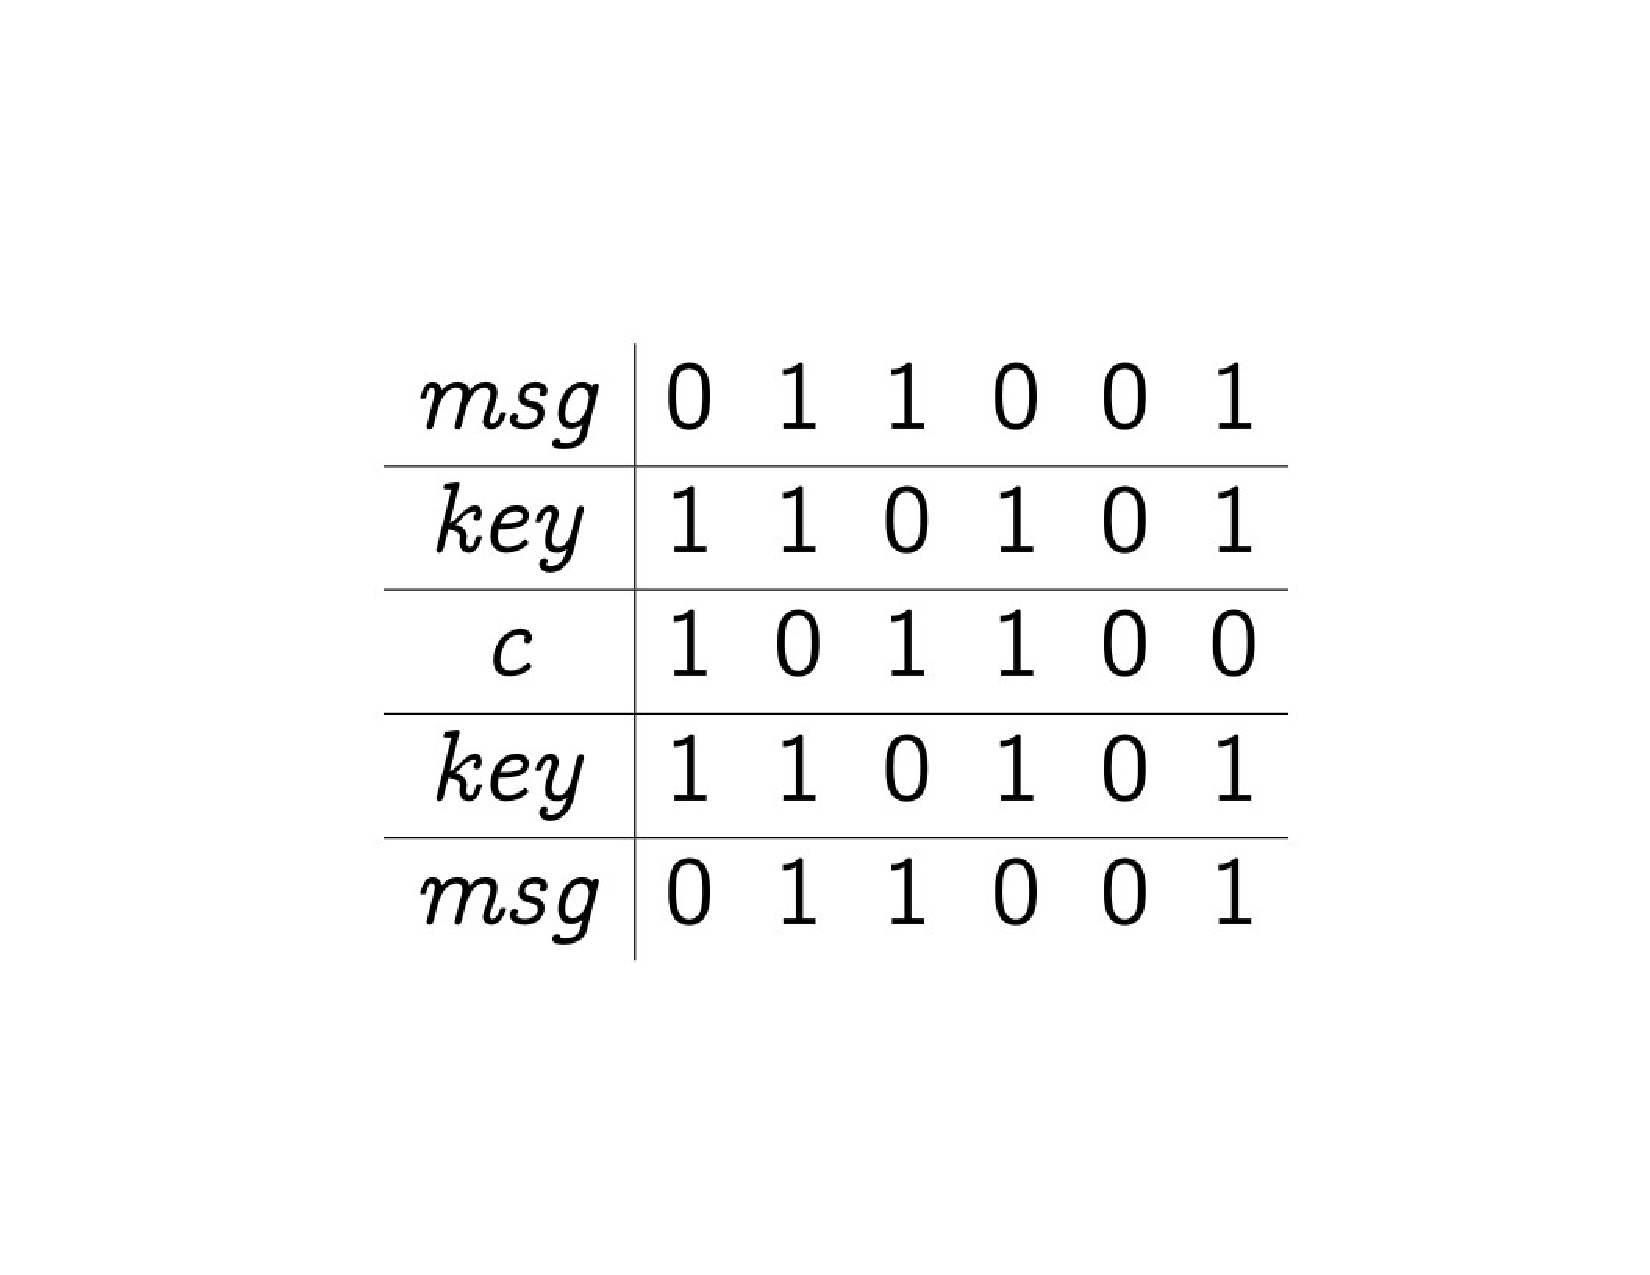
\includegraphics[width=\textwidth]{img/example_img.pdf}
\caption{L'interfaccia \texttt{GLaDOS}.}
\label{img:example}
\end{figure}

\section{Altra sezione}

\textbf{Sottotesto in grassetto}.

\subsection*{Esempio minimale}

\subsubsection{Sotto sotto sezione con paragrafi}

\paragraph{Paragrafo1} Contenuto.

\paragraph{Paragrafo Risposta 1} Contenuto \textit{paragrafo}, con riferimento immagine
\Cref{img:example}: e anche \texttt{Scrittura unicode}.

\chapter{Capitolo 3}
\section{Sezione}

Contenuto

\subsection{Esempio con sottosezioni e permalink}

\subsubsection{Utilizzo di \texttt{LoadingCache} dalla libreria Google Guava}

Permalink: \url{https://github.com/AlchemistSimulator/Alchemist/blob/d8a1799027d7d685569e15316a32e6394632ce71/alchemist-incarnation-protelis/src/main/java/it/unibo/alchemist/protelis/AlchemistExecutionContext.java#L141-L143}

\subsubsection{Utilizzo di \texttt{Stream} e lambda expressions}

Usate pervasivamente. Il seguente è un singolo esempio.
Permalink: \url{https://github.com/AlchemistSimulator/Alchemist/blob/d8a1799027d7d685569e15316a32e6394632ce71/alchemist-incarnation-protelis/src/main/java/it/unibo/alchemist/model/ProtelisIncarnation.java#L98-L120}

\subsubsection{Scrittura di metodo generico con parametri contravarianti}

Permalink: \url{https://github.com/AlchemistSimulator/Alchemist/blob/d8a1799027d7d685569e15316a32e6394632ce71/alchemist-incarnation-protelis/src/main/java/it/unibo/alchemist/protelis/AlchemistExecutionContext.java#L141-L143}

\nocite{*}
\bibliographystyle{plain}
\bibliography{report-template}

\end{document}
